
Over the past 100 years, roads have become more and more congested. The number of vehicles on the road in the UK alone has increased by more than 50\% since 1994\cite{AllVehiclesVEH01}, this is thought to be considerably higher in developing countries, and the trend over the past decade is a 1-2\% growth year-on-year. This can be seen in Figure~\ref{fig:vehicles-time}. All the while, road networks in countries such as the UK are not being extended, putting the existing infrastructure under increasing strain.

On top of this, human controlled vehicles do not efficiently utilise the roads available, requiring additional space per vehicle due to factors such as \textit{reaction time}, if we were able to remove these human elements it would be possible to greatly increase the throughput of the same amount of road infrastructure.

We can also consider the impact of autonomous navigation on road fatality rates. Over the past 10 years there have been an average of 1984 deaths per year on UK roads\cite{ReportedRoadCasualties}, with around a further 24,000 people seriously injured. Many of these incidents will have occurred due to human error, error which could be eliminated if the human factor were to be removed from vehicle navigation and routing and replaced with a robust, reliable automated system.

Many common approaches to solving this problem rely on directly replacing each human driver with an artificially intelligent system, examples of such systems include Tesla's autopilot or Google's \textit{Waymo} taxi service. These are designed to plan and primarily consider a single vehicle. By taking this approach, these systems still have to account for this \textit{human factor}, reducing much, if not all, efficiency gains.

In this paper, a more totalitarian system is proposed, designed and evaluated in which every agent is working to reduce the \textbf{net} travel time of the system, whilst strictly enforcing safety guarantees by avoiding collisions and infeasible space.


\begin{figure}[ht]
  \centering
  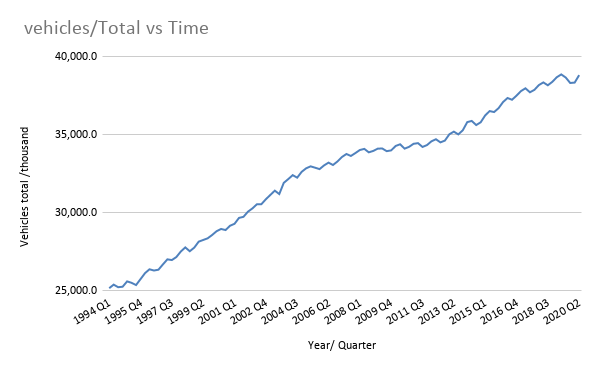
\includegraphics[scale=0.5]{figures/vehicles-time.png}
  \caption{\label{fig:vehicles-time} Total vehicles registered on UK roads over time\cite{AllVehiclesVEH01}}
\end{figure}


\section{Goals}

The overarching goal of this project is to optimally route traffic in the setting of a fully-autonomous road system. This however, is an aspirational goal with many sub-requirements to be fulfilled before it can come to fruition.

Here an \textit{optimal} route is defined as the shortest possible path between two given points such that, it does not pass through infeasible space or collide with any other routes which may be executed concurrently. In reality, due to time and technical constraints, despite the Genetic Algorithms being \textit{probabilistically optimal}, we will relax this requirement to be the \textit{best}, or shortest route which still conforms to these constraints and is found within a certain number of generations over a population of a given size.

Initially, we want to be able to route a single agent through a single stretch of road, avoiding any and all infeasible space present within the road's boundaries whilst also staying within these boundaries at all times.

This will require the definition of an individual encoding in both the phenotypic and genotypic spaces (See Section~\ref{sec:back:GAs}) along with corresponding genetic operators which can operate on the individuals genotypic structure.

Building on this, the next sub-goal will be to create multiple routes with these characteristics whilst adding the requirement that none
of them collide with each-other.

This will require a notion of velocity in order to accurately extrapolate the position along a route an agent is at a given point in time. This will also require the ability to detect if and where two routes intersect.

Finally, we need to wrap this functionality in such a way that allows for agents to navigate through multiple stretches of road, connected via intersections, with each sub-route maintaining all the requirements of the solutions to the previous sub-problems.

Formal definitions of these goals can be seen in Problems~\ref{prob:Spec},\ref{prob:sub1} and~\ref{prob:sub2}

\begin{figure}[htpb]
    \centering
    \begin{problem}{prob:Spec}

        \problemtitle{Top-level Goal}
        \probleminput{ 
            \begin{itemize}
                \item A road system $\mathcal{R}$ represented as a graph $\mathcal{R} = (V,E)$


                    Where each edge $e \in E$ is a section of road defined as the space between two vertices $v^1,v^2 \in V$ which is bounded by two functions $b_1(x)$ and $b_2(x)$ and augmented by a set of obstacles $O$ representing infeasible sections of road space
                \item a set of agents, $A = \left\{ a_1,\ldots,a_n \right\}$
                \item a list of vertex pairs representing start and goal points for each agent:

                    $\mathcal{V} = \left\{ (v_1^1,v_1^2),\ldots, (v_n^1, v_n^2) \right\}, v_{i \in [1 \ldots n]}^{j \in [1,2]} \in V$

                where the route for agent $a_i$ is from vertex $v_i^1$ to $v_i^2$
            \end{itemize}
        }
        \problemquestion{ What is the set of optimal routes $\mathcal{V}_{optimal}$, where the $i^{\text{th}}$ element  is defined as a set of linked Bézier curves connecting $v_i^1$ and $v_i^2$ through feasible space?}
        \end{problem}
\end{figure}

\begin{figure}[htpb]
    \centering
    \begin{problem}{prob:sub1}
        \problemtitle{Sub-Goal: Cooperative route planning}
        \probleminput{
            \begin{itemize}
                \item A start point $P_{start}$ and a goal point $P_{goal}$ 
                \item A section of road as defined in Problem~\ref{prob:Spec}
                \item A knowledge of all routes being planned to be executed concurrently.
            \end{itemize}
        }
        \problemquestion{What is the optimal route, in the form of a Bézier curve, between these two points s.t. it does not collide with any other agents or pass through any infeasible regions in the road space?}
    \end{problem}
\end{figure} 

\begin{figure}[htpb]
    \centering
    \begin{problem}{prob:sub2}
        \problemtitle{Sub-Goal: Single agent route planning}
        \probleminput{
            \begin{itemize}
                \item A start point $P_{start}$ and a goal point $P_{goal}$ 
                \item A section of road as defined in Problem~\ref{prob:Spec}
            \end{itemize}
        }
        \problemquestion{What is the optimal route, in the form of a Bézier curve, between these two points s.t. it does not pass through any infeasible regions in the road space?}
    \end{problem}
\end{figure} 


\subsection{Requirements}
\label{subsec:requirements}

The goal of this project was not to produce a production-ready system, but instead, to investigate the plausibility of GAs on the real future possibility of completely autonomous road networks. As such I feel it useful to outline the theoretical requirements of a production grade system. To do this formally I will employ Propositional and Temporal logic.

\begin{enumerate}
\item The system should never return a set of routes such that, for any time $t , \forall i \in [1,n], \forall j \in [1,n], j \neq i, I_{i}(t) = I_{j}(t)$. I.e. for any time, no routes should inhabit the same point, meaning there are no collisions in the planned routes. Where $I_{i}(t)$ is the position of agent $i$ at time $t$ and $n$ is the number of agents being planned for.

  \item The system should never return a set of routes such that, for any time $t , \forall i\in [1,n], \forall o \in O, I_{i}(t) \notin o$, I.e. for any time, no routes should pass through and infeasible space defined by any obstacles, $o\in O$.
\end{enumerate}

%TC:macro \todo 1

%%% Local Variables:
%%% mode: latex
%%% TeX-master: "report"
%%% End:
